
%%% Exercise 1 %%%

\exercise{Different paths\label{ExHobbitPaths}}{1}
%\hint{Level 1}{Try quickly.}
Decide which of the following is an open walk / closed walk / trail / path / circuit / cycle in the network shown below.
\begin{center}
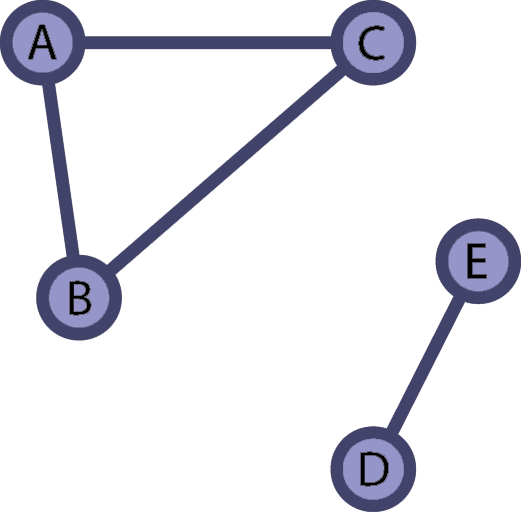
\includegraphics[width=0.2\textwidth]{HobbitSmall2.png}
\end{center}

\subquestion A,(A,C),C,(C,B),B;
\solution
An open walk, a trail and a path. 

\subquestion A,(A,B),B,(A,C),A; 
\solution
This isn't any walk because B is followed by (A,C) in the sequence, which does not contain B as an endpoint. 

\subquestion 
A,(A,B),B,(B,C),C,(A,C),A; 
\solution
A closed walk, also a circuit and a cycle. 
 
\subquestion 
A,(A,D),D,(A,D),A; 
\solution
This isn't any walk because (A,D) isn't an edge.

\subquestion 
A,(A,C),C,(B,C),B,(B,A),A,(A,C),C,(A,C),A; 
\solution
A closed walk, it isn't a circuit or cycle because (A,C) is used multiple times. 

\subquestion 
B,(A,B),A,(A,C),C.
\solution
An open walk, trail and path.
\solutionend


